\documentclass[10pt]{beamer}

\usetheme[progressbar=frametitle]{metropolis}
\usepackage{appendixnumberbeamer}

\usepackage{booktabs}
\usepackage[scale=2]{ccicons}

\usepackage{verbatim}
\usepackage[utf8]{inputenc}
\usepackage{listings}

\usepackage{array}

\usepackage{lipsum}
\usepackage{setspace}
%\usepackage{xcolor}

\usepackage{pgfplots}
\usepgfplotslibrary{dateplot}

\DeclareMathOperator{\Tr}{Tr}

\usepackage{mathbbol}

\usepackage{xspace}
\newcommand{\themename}{\textbf{\textsc{metropolis}}\xspace}

\title{Software Development and Parallel Computing with C++ -- Class 1 (part 1)}
%\subtitle{A modern beamer theme}
% \date{\today}
\date{}
\author{Gustavo Ram{\'i}rez}
%\institute{Center for modern beamer themes}
% \titlegraphic{\hfill\includegraphics[height=1.5cm]{logo.pdf}}

\begin{document}

\maketitle

%\begin{frame}{Tabla de contenidos}
%  \setbeamertemplate{section in toc}[sections numbered]
%  \tableofcontents[hideallsubsections]
%\end{frame}



\section{Brief intro to C}


\begin{frame}[fragile]{What is C?}
\begin{itemize}
\item procedural, imperative computer programming language
\item developed in 1972 by Dennis M. Ritchie
\item essentially all UNIX application programs have been written in C
\item formalized in 1988 by ANSI (American National Standards Institute)
\end{itemize}
\end{frame}


\begin{frame}[fragile]{Why C first?}
\begin{itemize}
\item contains/represents the basics for other programming languages (C++, ...)
\item most courses in C++ assume C knowledge
\item depending on what you're doing, you could use only C and not go into C++ or any other OOP language
\end{itemize}
\end{frame}



\begin{frame}[fragile]{How to learn it (C)?}
\begin{itemize}
\item plenty of online material
\item good source: www.tutorialspoint.com
\item do things \textbf{on your own}!
\end{itemize}
\end{frame}


\begin{frame}[fragile]{Why is it so widely used?}
\begin{itemize}
\item easy to learn
\item structured
\item efficient (programs)
\item can handle low-level activities
\item its compilation is cross-platform
\end{itemize}
\end{frame}


\begin{frame}[fragile]{What we'll cover (today)}
\begin{itemize}
\item basic structure of a program
\item compilation and execution
\item variables and types
\item functions (within 'main')
\item \textit{\#include} guards and \textit{\#pragma once}
\item arrays
\item pointers
\item structs
\item control statements
\end{itemize}
\end{frame}

\begin{frame}[fragile]{Basic structure of a C program}
\begin{lstlisting}
/* Lines beginning with # are directives read and
   interpreted by what is known as the preprocessor */
#include <stdio.h>

int main()
{
  //print msg on screen
  int i=15;
  printf("Hola, World!\n");
  printf("Value of i: %d\n", i);
  return 0;  //0 represents a successful execution and
             //return of the program
}
\end{lstlisting}
\end{frame}


\begin{frame}[fragile]{Compilation and execution}
\begin{itemize}
\item save the code in a file named program\_basic.c (or whatever name you want)
\item compilation:
\begin{lstlisting}
gcc program_basic.c -o program_basic
\end{lstlisting}
\item execution:
\begin{lstlisting}
./program_basic.c
\end{lstlisting}
\end{itemize}
\end{frame}


\begin{frame}[fragile]{Variables and types}

Declaration of a variable:

\begin{lstlisting}
TYPE IDENTIFIER1, IDENTIFIER2, ...;
\end{lstlisting}

Types of types:

\begin{center}
  \renewcommand{\arraystretch}{1.7}
  %\begin{adjustwidth}{-3cm}{}
  \vspace{-1.8em}%
  %\hspace{-1.5em}%
  \begin{tabular}{ | c | m{2cm} | m{8cm} | }
    \hline
    1 & Basic types & They are arithmetic types and are further classified into: (a) integer types and (b) floating-point types. \\ \hline
    2 & Enumerated types & They are again arithmetic types and they are used to define variables that can only assign certain discrete integer values throughout the program. \\ \hline
    3 & The type void & The type specifier void indicates that no value is available. \\ \hline
    4 & Derived types & They include (a) Pointer types, (b) Array types, (c) Structure types, (d) Union types and (e) Function types. \\
    \hline
  \end{tabular}
\end{center}

\end{frame}


\begin{frame}[fragile]{Typedef}

Syntax:

\begin{lstlisting}
typedef OLD_TYPE NEW_NAME;
\end{lstlisting}

Example:

\begin{lstlisting}
typedef unsigned int BARE_INT;
\end{lstlisting}
\end{frame}


\begin{frame}[fragile]{Getting info from data types}
\begin{lstlisting}[
    basicstyle=\scriptsize, %or \small or \footnotesize etc.
]
#include <stdio.h>
#include <limits.h> // for int
#include <float.h>  // for float
#include <math.h>   // for pow(...)

int main() {
  printf("INFO - unsigned int\n");
  printf("Storage size for int: %d bytes \n", sizeof(unsigned int));
  printf("Range: %d - %d", 0, pow(2, sizeof(unsigned int))-1);

  printf("\nINFO - float\n");
  printf("Storage size for float : %d \n", sizeof(float));
  printf("Minimum float positive value: %E\n", FLT_MIN );
  printf("Maximum float positive value: %E\n", FLT_MAX );
  printf("Precision value: %d\n", FLT_DIG );

  return 0;
}
\end{lstlisting}
\end{frame}






\begin{frame}[fragile]{Functions}

General form:

\begin{lstlisting}[
    basicstyle=\scriptsize, %or \small or \footnotesize etc.
]
return_type function_name( parameter list ) {
   body of the function
}
\end{lstlisting}

Specific example:

\begin{lstlisting}[
    basicstyle=\scriptsize, %or \small or \footnotesize etc.
]
#include <stdio.h>

//Function declaration
void print_map_elem(char, int);
//Alternative declaration
//void print_map_elem(char key, int val);

int main()
{
  print_map_elem('k', 5);
  return 0;
}

//Full implementation of the function
void print_map_elem(char key, int val) //key and val are called 'formal parameters'
{
  printf("Pair: %c, %d\n", key, val);
}
\end{lstlisting}
\end{frame}




\begin{frame}[fragile]{Static variables}
\begin{lstlisting}[
    basicstyle=\scriptsize, %or \small or \footnotesize etc.
]
#include <stdio.h>

/* The x variable will be redefined to 123 each time
   that f() is called */
void f(){
  int x=123;
  x++;
  printf("f(): x=%d\n",x);
}

/* The use of 'static' makes x accessible globally, and the line
   'static int x=123;' is called only once i.e. the first time that
   g() is called */
void g(){
  static int x=123;
  x++;
  printf("g(): x=%d\n",x);
}

int main(){
  //non-incremental calls
  f(); f(); f();
  //incremental calls
  g(); g(); g();
}
\end{lstlisting}
\end{frame}


\begin{frame}[fragile]{\textit{\#include} guards and \textit{\#pragma once}}

Check files:

\begin{lstlisting}
program_pragma_once.c
program_pragma_once_level1.h
program_pragma_once_level2.h

program_include_guards.c
program_include_guards_level1.h
program_include_guards_level2.h
\end{lstlisting}

@ ../../examples\_miscellaneous/
\end{frame}


\begin{frame}[fragile]{Arrays}
Declaration:

\begin{lstlisting}
type arrayName [ arraySize ];
\end{lstlisting}

Example:

\begin{lstlisting}[
    basicstyle=\footnotesize, %or \small or \footnotesize etc.
]
...
#define LENGTH 5
double array_doubles[LENGTH] = \
    {10.0, 2.3, 5.4, 8.9, 3.3}; /* The number of values between
                                braces { } cannot be larger
                                than the number of elements that
                                we declare for the array
                                between square brackets [ ] */
//Alternatively
double array_doubles[] = {10.0, 2.3, 5.4, 8.9, 3.3};
...
\end{lstlisting}

Access:

\begin{lstlisting}
double third_elem = array_doubles[2];
\end{lstlisting}
\end{frame}


\begin{frame}[fragile]{Passing arrays to functions}
\begin{lstlisting}
void myF(int params[], int size)
{
  ...
}
\end{lstlisting}
\end{frame}


\begin{frame}[fragile]{Return array from function}
\begin{lstlisting}
int *myF(...)
{
  ...
  /* If the array is created within the function,
     use static */
  static int array_o[17];
  ...
  return array_o;
}
\end{lstlisting}
\end{frame}


\begin{frame}[fragile]{Pointers}
Let's print the address of a memory location:

\begin{lstlisting}[
    basicstyle=\footnotesize, %or \small or \footnotesize etc.
]
#include <stdio.h>

int main()
{
  int test_arr[] = {2,3,7};

  printf("Value of second element: %d\n", test_arr[1]);
  printf("Address of second element: %p\n", &(test_arr[1]));
  printf("Address of second element: %p\n", test_arr+1);

  return 0;
}
\end{lstlisting}

Declaration of a pointer: TYPE *IDENTIFIER = ADDRESS;
\end{frame}


\begin{frame}[fragile]{Pointers}

Alternatively:

\ \\

\begin{lstlisting}[
    basicstyle=\scriptsize, %or \small or \footnotesize etc.
]
#include <stdio.h>
#include <stdlib.h> //to enable malloc(...)

int main()
{
  int *p_arr;

  p_arr = (int*) malloc(3*sizeof(int));

  p_arr[0] = 2;
  *(p_arr+1) = 3;
  p_arr[2] = 7;

  printf("Value of second element: %d\n", p_arr[1]);
  printf("Address of second element: %p\n", &(p_arr[1]));
  printf("Address of second element: %p\n", p_arr+1);

  free(p_arr);

  return 0;
}
\end{lstlisting}
\end{frame}


\begin{frame}[fragile]{Pointers (to pointers!)}
In the previous example, one could do:

\begin{lstlisting}
...
int **p_p_arr = &p_arr; /* Pointer pointing to
                           a pointer */
...
\end{lstlisting}
\end{frame}


\begin{frame}[fragile]{Pointers}
Check:

\begin{lstlisting}
program_pointers.c
\end{lstlisting}

@ ../../examples\_miscellaneous/
\end{frame}


\begin{frame}[fragile]{Pointers}
Check:
\begin{lstlisting}
program_pointers_functions.c
\end{lstlisting}

@ ../../examples\_miscellaneous/
\end{frame}


\begin{frame}[fragile]{Control Statements: if}

Syntax:

\ \\

\begin{lstlisting}[
    basicstyle=\footnotesize, %or \small or \footnotesize etc.
]
if(CONDITION1)
{
  
}
else if(CONDITION2)
{
  /* STATEMENTS */
}
...
/* MORE else if STATEMENTS HERE */
...
else
{
  /* STATEMENTS */
}
\end{lstlisting}
\end{frame}


\begin{frame}[fragile]{Control statements: if}

Besides if: while, do while, the ternary ? operator, switch, for. We'll only cover if and for here.

\ \\

The C programming language assumes any non-zero and non-null values as true, and if it is either zero or null, then it is assumed as false value.

\end{frame}

\begin{frame}[fragile]{Command Line Arguments}

Compilation and execution again:

\ \\

\begin{lstlisting}
gcc program.c -o program

./program inp1 inp2 ...
\end{lstlisting}
\end{frame}


\begin{frame}[fragile]{Command Line Arguments}

Example:

\ \\

\begin{lstlisting}[
    basicstyle=\footnotesize, %or \small or \footnotesize etc.
]
#include <stdio.h>

int main(int argc, char *argv[]){  //The second argument can be
                                   //written as: char **argv
  if(argc == 2) {
    printf("The argument supplied is %s\n", argv[1]);
  }
  else if(argc > 2)
  {
    printf("Too many arguments supplied.\n");
  }
  else{
    printf("One argument expected.\n");
  }

  return 0;
}
\end{lstlisting}
\end{frame}


\begin{frame}[fragile]{Command Line Arguments: memory}
\begin{figure}[h]
    \centering
    \hspace*{-1.1cm}
    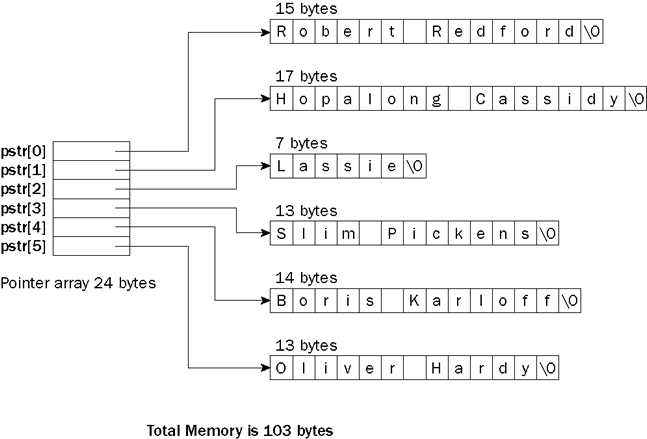
\includegraphics[width=1.05\textwidth]{char_p_p}
    %\caption{example of construction of the rows of $M$ corresponding to the point labeled as "2" using a $4{\times}4$ lattice.}
    \label{fig:2d_lattice_into_matrix}
\end{figure}
\end{frame}


\begin{frame}[fragile]{Control Statements: for}

Syntax:

\ \\

\begin{lstlisting}
TYPE VAR;
for(INIT; CONDITION; EXEC)
{
  
}
\end{lstlisting}

where:

\begin{itemize}
\item INIT: initialisation of VAR (or any other necessary initialisations)
\item CONDITION: when this condition is met, the loop stops and exits
\item EXEC: something that is executed on each iteration
\end{itemize}
\end{frame}


\begin{frame}[fragile]{Control Statements: for}

Example:

\begin{lstlisting}[
    basicstyle=\footnotesize, %or \small or \footnotesize etc.
]
...
int i;
for(i=0; i<10; i++)
{
  printf("Iteration: %d\n", i);
}
...
\end{lstlisting}

Commands per iteration in the previous example:

\begin{lstlisting}[
    basicstyle=\footnotesize, %or \small or \footnotesize etc.
]
------------------------------------------------------
Iter    Commands
------------------------------------------------------
1       initialize i=0, check i<10, call printf(...),
        increment: i++
2       check i<10, call printf(...), increment: i++
3       check i<10, call printf(...), increment: i++
...
11      check i<10, break
------------------------------------------------------
\end{lstlisting}

\end{frame}


\begin{frame}[fragile]{Extension of Command Line Args using for}
\begin{lstlisting}[
    basicstyle=\scriptsize, %or \small or \footnotesize etc.
]
#include <stdio.h>

int main(int argc, char *argv[]){  //The second argument can be
                                   //written as: char **argv
  if(argc == 2) {
    printf("The argument supplied is %s\n", argv[1]);
  }
  else if(argc > 2)
  {
    printf("The arguments supplied are: ");
    int i;
    for(i=1; i<argc-1; i++)
    {
      printf("%s, ", argv[i]);
    }
    printf("%s\n", argv[argc-1]);
  }
  else{
    printf("One argument expected.\n");
  }

  return 0;
}
\end{lstlisting}
\end{frame}


\begin{frame}[fragile]{Structs}

Syntax:

\begin{lstlisting}
struct [structure tag] {

   member definition;
   member definition;
   ...
   member definition;
} [one or more structure variables];
\end{lstlisting}
\end{frame}


\begin{frame}[fragile]{Structs}

Let's say we want to avoid passing an array like this:

\begin{lstlisting}[
    basicstyle=\scriptsize, %or \small or \footnotesize etc.
]
#include <stdio.h>

void print_arr(int params[], int size)
{
  int i;

  printf("Array: ");
  for(i=0; i<size-1; i++)
  {
    printf("%d, ", params[i]);
  }
  printf("%d\n", params[size-1]);
}

int main()
{
  int arr_i[] = {2, 3, 5, 89};
  const int size = 4;

  print_arr(arr_i, size);
}
\end{lstlisting}

and we want to pass it as a single structure. Use a struct!
\end{frame}


\begin{frame}[fragile]{Structs}
\begin{lstlisting}[
    basicstyle=\tiny, %or \small or \footnotesize etc.
]
#include <stdio.h>
#include <stdlib.h>

struct arr_ints{
  int size; int *data;
};

//Redefine the name of the struct
typedef struct arr_ints ARR_INTS_P;

void print_arr(ARR_INTS_P arr_pack_x)
{
  int i;
  printf("Array: ");
  for(i=0; i<arr_pack_x.size-1; i++)
  {
    printf("%d, ", arr_pack_x.data[i]);
  }
  printf("%d\n", arr_pack_x.data[arr_pack_x.size-1]);
}

int main()
{
  ARR_INTS_P arr_pack;

  arr_pack.size = 4;
  arr_pack.data = (int*) malloc(arr_pack.size * sizeof(int));

  (arr_pack.data)[0] = 2; (arr_pack.data)[1] = 3; (arr_pack.data)[2] = 5; (arr_pack.data)[3] = 89;

  print_arr(arr_pack);
  free(arr_pack.data);
  return 0;
}
\end{lstlisting}
\end{frame}


\begin{frame}[fragile]{Final comments}

There are many things we didn't cover today. Go and check ../notes.pdf for a more thorough intro to C!

\end{frame}


\begin{frame}[fragile]{End}
End.
\end{frame}



\end{document}

